\begin{frame}[t,fragile]{Ausgangspunkt}
\begin{itemize}
\item Betriebswirtschaftliche Software
\item Extrem schlechte Codequalität (sowohl messbar als auch erfahrbar)
\item Funktionalität eines Moduls musste verändert werden
\begin{itemize}
\item Bugfixing
\item neue Features
\item bessere Tests
\end{itemize}
\end{itemize}

$\Rightarrow$ Wir mussten einen Umbau vornehmen
\end{frame}

\begin{frame}[t,fragile]{Vorhandene Codestruktur}
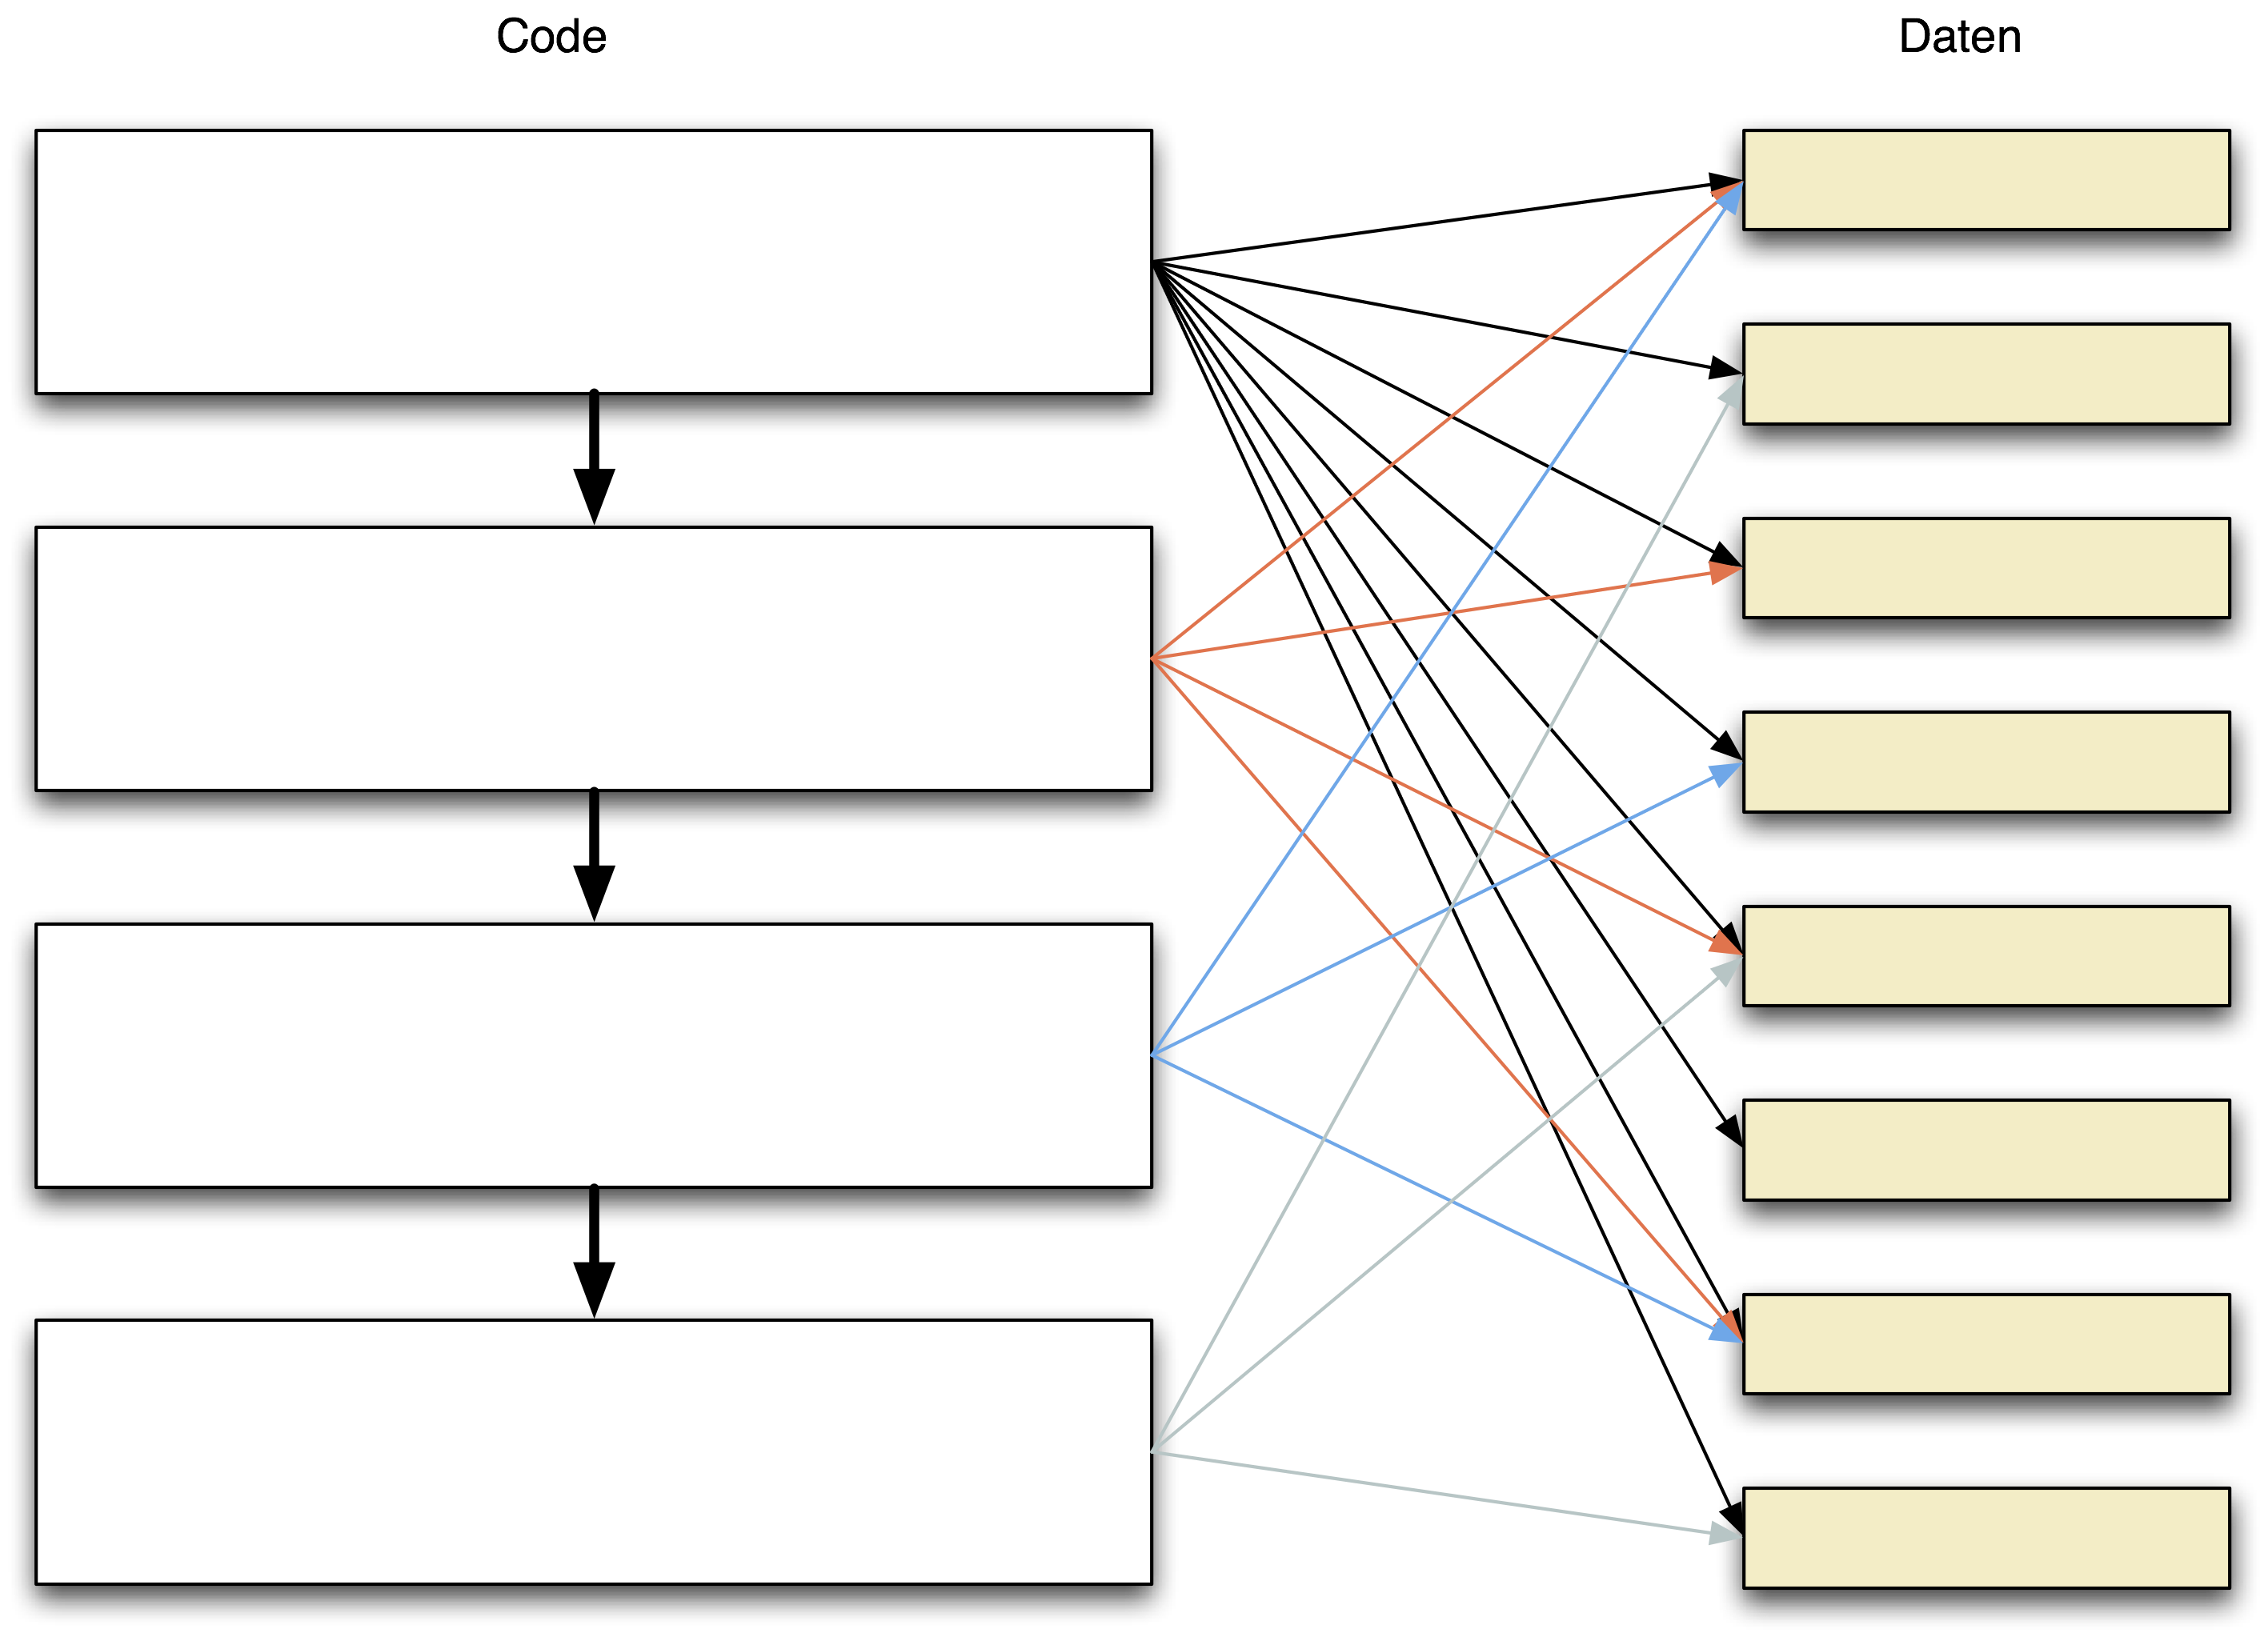
\includegraphics[width=.8 \paperwidth]{Codestruktur.png}
\end{frame}

\begin{frame}[t,fragile]{Probleme der vorhandenen Codestruktur}
\begin{itemize}
\item Code schreibt Werte in separate Datenobjekte (\glqq Push\grqq{})
\item Mehrfache Schreibzugriffe auf denselben Wert
\item Codeteile greifen auf vorher geschriebene Werte zu
\item Code ist getrieben vom Blick von innen: Was muss ich alles in Summe tun, um eine Menge von Ergebnissen abliefern zu können?
\end{itemize}
\end{frame}



\begin{frame}[t,fragile]{Unser Ansatz}
\begin{itemize}
\item Annahmen:
\begin{itemize}
\item Der alte Code ist großteils inkorrekt und lückenhaft
\item Es existiert umfassendes Wissen über die gewünschte Fachlogik
\end{itemize}

\item Entschluss:
\begin{itemize}
\item Neuimplementierung auf der grünen Wiese (mit Feature-Toggle)
\item Erstellung neuer Tests anhand der parallel zu definierenden Fachlichkeit
\item Kontinuierliche Anpassung der vorhandenen Tests
\end{itemize}
\end{itemize}

\end{frame}


\begin{frame}[t,fragile]{Unsere Erfahrungen}
\begin{itemize}
\item Probleme:
\begin{itemize}
\item Die Ausarbeitung der fachlichen Spezifikation ist viel komplizierter und aufwändiger als gedacht
\item Abweichungen zum alten Code sind schwer zu analysieren
\item Die Testabdeckung ist zu gering $\Rightarrow$ Wir übersehen relevante Fälle 
\end{itemize}
\end{itemize}

\begin{itemize}
\item Ursachen:
\begin{itemize}
\item Falsche Annahmen
\item Vermischung von Umbau und Änderung
\item Arroganz (\glqq Wir wissen es besser als unsere Vorgänger\grqq{})
\end{itemize}
\end{itemize}

$\Rightarrow$ Wir sind den Umbau viel zu naiv angegangen

\end{frame}


%\begin{frame}[t,fragile]{}
%\begin{itemize}
%\item
%\end{itemize}
%\end{frame}
%
%\begin{frame}[t,fragile]{}
%\begin{itemize}
%\item
%\end{itemize}
%\end{frame}
%
%\begin{frame}[t,fragile]{}
%\begin{itemize}
%\item
%\end{itemize}
%\end{frame}
%
%\begin{frame}[t,fragile]{}
%\begin{itemize}
%\item
%\end{itemize}
%\end{frame}

\begin{frame}[t,fragile]{Wie geht es besser?}
\begin{itemize}
\item Vor dem Umbau Fakten sammeln, Annahmen allein genügen nicht
\begin{itemize}
\item Wie hoch ist die Testabdeckung? (Coverage)
\item Welche Fälle werden fachlich durch vorhandene Tests abgedeckt?
\item Existiert eine Spezifikation?
\item Ist diese synchron mit dem vorhandenen Code?
\end{itemize}

\item Grundsätzlich gilt: Im Zweifel hat der vorhandene Code Recht!

\item Keine Änderungen an der Logik während des strukturellen Umbaus!

\item Explizite Abnahme des Umbaus
\begin{itemize}
\item Alle automatisierten Tests laufen
\item Alle manuellen Tests laufen
\item Alle bekannten Bugs werden geprüft
\item Jede Verhaltensabweichung muss begründet werden
\end{itemize}

\end{itemize}
\end{frame}



\begin{frame}[t,fragile]{Wozu das Ganze?}
\begin{itemize}
\item Umbau der Struktur: damit die vorhandene Implementierung der Sachlichkeit besser sichtbar wird und isoliert vorliegt
$\Rightarrow$ ermöglicht später gezielte Änderung einzelner Aspekte der Fachlichkeit
\item Trennung der Aspekte: damit die Regressionstests bei den Strukturveränderungen gültig bleiben und alle Veränderungen im Verhalten anzeigen
\item Fachlich motiviert, Blick von außen aus Sicht der Ergebnisse:
\begin{itemize}
\item Welche Werte will ich haben?
\item Wie berechnet sich welcher Wert?
\item Welche Arten von Ergebniswerten gibt es? Gemeinsamkeiten, Unterschiede?
\end{itemize}
\end{itemize}
\end{frame}


\begin{frame}[t,fragile]{Ideale Vorgehensweise}
\begin{itemize}
\item Feature-Toggle zum Vergleichen der alten und der neuen Version
\item Identifikation bzw. Schaffen eines minimalen Eingriffspunkts
\item Beibehalten der externen API an diesem Eingriffspunkt

\item Umbau:
\begin{itemize}
\item Fachlich motiviert
\item Rein strukturell
\end{itemize}

\item Ziel:
\begin{itemize}
\item Separation of Concerns
\item On-Demand-Ermittlung aller Werte (\glqq Pull\grqq{})
\item Werte-Caching mittels Lazy-Initialization
\end{itemize}

\end{itemize}
\end{frame}




\begin{frame}[t,fragile]{Umbau: Vorbereitung}
\begin{itemize}
\item Existierenden Code duplizieren
\item Feature Toggle an den Aufrufstellen einbauen
\end{itemize}
\end{frame}
 
\begin{frame}[t,fragile]{Vorarbeiten}
\begin{itemize}
\item Java-Datumsarithmetik kapseln, z.~B.
\begin{itemize}
\item Joda Time
\item Eigene Klassen
\end{itemize}
\item Namensgebung von Variablen verbessern
\end{itemize}
\end{frame}

\begin{frame}[t,fragile]{Strukturellen Code isolieren}
\begin{itemize}
\item Inline method: Nur noch eine Methode
\item Schleifen über Ergebnisstruktur nach außen bringen
\item Schleifen vereinheitlichen
\end{itemize}
\end{frame}

\begin{frame}[t,fragile]{Aspekte isolieren}
\begin{itemize}
\item Schleifenrumpf in eigene Klasse mit einer Methode extrahieren
\item Pro Ergebniswert ein Duplikat dieser Methode
\item Jeweils Irrelevantes aus den Methoden entfernen
\end{itemize}
\end{frame}

\begin{frame}[t,fragile]{Zielstruktur aufbauen}
\begin{itemize}
\item Zuerst nur als Gerüst mit Befüllung von außen
\item Berechnung \textbf{eines} Werts in die Zielstruktur übertragen
\item Prüfen der Tragfähigkeit der Zielstruktur
\end{itemize}
\end{frame}

\begin{frame}[t,fragile]{Vervollständigung}
\begin{itemize}
\item Wert für Wert in die Zielstruktur übertragen
\item Parallel dazu Unit-Tests aufbauen
\item Refactoring: 
\begin{itemize}
\item Extrahieren von Methoden
\item Zusammenfassen gleicher Funktionalität
\item Generelle Aufräumarbeiten
\end{itemize}
\item Klärung fachlicher Unklarheiten, Korrektur der Logik
\end{itemize}
\end{frame}

%\begin{frame}[t,fragile]{}
%\begin{itemize}
%\item
%\end{itemize}
%\end{frame}
%
%\begin{frame}[t,fragile]{}
%\begin{itemize}
%\item
%\end{itemize}
%\end{frame}
%
%\begin{frame}[t,fragile]{}
%\begin{itemize}
%\item
%\end{itemize}
%\end{frame}
%
%\begin{frame}[t,fragile]{}
%\begin{itemize}
%\item
%\end{itemize}
%\end{frame}
%
%\begin{frame}[t,fragile]{}
%\begin{itemize}
%\item
%\end{itemize}
%\end{frame}

